\begin{figure}[t]
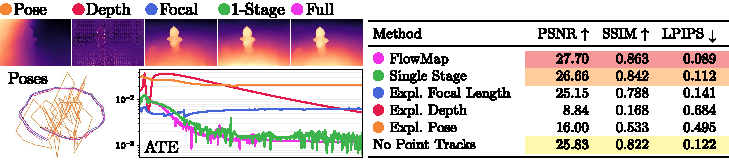
\includegraphics{figures/ablations/fig_ablations_pdf.pdf}



\caption{
\textbf{Ablations.}
We ablate the proposed feed-forward re-parameterizations of depth, pose, and intrinsics across all datasets.
We find that these reparameterizations are not only critical for high-quality downstream 3D Gaussian Splatting, but also lead to dramatically accelerated convergence, where FlowMap generally converges to high quality poses within a fraction of the optimization steps required for the ablated variants.
We further find that point tracks lead to a significant boost over optical flow alone (right).
See the supplemental document for more ablations.
\vspace{-10pt}
}
\label{fig:ablations}
\end{figure}
